\documentclass[conference,10pt]{IEEEtran}
\usepackage{fontspec}
\setmainfont[Path={fonts/},BoldFont=timesbd.ttf,ItalicFont=timesi.ttf,BoldItalicFont=timesbi.ttf]{times.ttf}
\makeatletter
\renewcommand\normalsize{\@setfontsize\normalsize{10}{12}}
\makeatother
\let\small\normalsize\let\footnotesize\normalsize\let\scriptsize\normalsize
\let\large\normalsize\let\Large\normalsize\let\LARGE\normalsize
\let\huge\normalsize\let\Huge\normalsize
\setlength{\tabcolsep}{3pt}
\normalsize
\usepackage{graphicx,booktabs,array,url}
\urlstyle{same}
\usepackage{amsmath}
\usepackage{microtype}
\hyphenation{AngioCAD CardioDiag}
\title{CARDIODIAG: Selection-Aware Evaluation, Calibration and Cross-Cohort Robustness for Retrospective Coronary Artery Disease Discrimination}
\author{\IEEEauthorblockN{Erukudinnela Akhil Preetham, Chunduri Hari Krishna, G Vennela}\IEEEauthorblockA{Department of Computer Science and Engineering\\Prasad V. Potluri Siddhartha Institute of Technology (PVPSIT)\\Vijayawada, Andhra Pradesh, India\\Project guide: K. Naga Gopi}}
\begin{document}
\pagestyle{plain}
\twocolumn[\begin{center}\normalsize\textbf{CARDIODIAG: Selection-Aware Evaluation, Calibration and Cross-Cohort Robustness for Retrospective Coronary Artery Disease Discrimination}\par\vspace{6pt}
Erukudinnela Akhil Preetham, Chunduri Hari Krishna, G Vennela\\
Department of Computer Science and Engineering\\
Prasad V. Potluri Siddhartha Institute of Technology (PVPSIT), Vijayawada, Andhra Pradesh, India\\
Project guide: K. Naga Gopi\end{center}\vspace{8pt}]
\thispagestyle{plain}
\begin{abstract}
High cardiovascular classification scores do not establish fair model comparisons, calibrated probabilities or cross-cohort reliability. We extend a CardioDiag-derived project through information-matched controls, selection-independent calibration and compatibility-constrained public-cohort evaluation. Z-Alizadeh Sani contains 303 source rows, including 216 CAD labels. Fifteen paired outer partitions compare historical selection with a 38-feature logistic control and independently calibrated ensembles. Mean source ROC-AUC was 0.9103 for selection and 0.9174 for equal-feature logistic regression. Fixed-C1 logit calibration improved the existing independent-calibration ensemble from AUC/Brier 0.9096/0.1037 to 0.9144/0.1029, while retaining lower AUC than identical uncalibrated components. A separate five-core model achieved source AUC 0.8059 and frozen-target AUC 0.7125 on 377 matched AngioCAD cases. Retrospective target-offset adaptation reduced held-out Brier from 0.1982 to 0.1507. Missingness augmentation improved performance under heavy random deletion but slightly degraded complete-input performance; typed encoding also regressed and was not promoted. A training-only 90\%-sensitivity threshold yielded held-out sensitivity 0.8889 and specificity 0.4904. Learning curves, coefficient bootstraps, input perturbations and exploratory decision curves quantify remaining sensitivities. Predictions, partitions, maps, hashes and tests preserve both positive and negative results. Previously examined cohorts, unresolved predictor timing, unverified patient independence and endpoint/coding differences preclude prospective or clinical-deployment claims. The contribution is an auditable retrospective reliability study rather than a universally superior diagnostic algorithm.
\end{abstract}
\noindent\textit{Final retrospective research report. Times New Roman, 10 point. Historical results and all negative comparisons are retained.}\par
\begin{IEEEkeywords}
Coronary artery disease, nested validation, calibration, external transport, information availability, reproducibility.

\end{IEEEkeywords}
\section{Introduction}
High cardiovascular classification scores do not establish fair model comparison, calibrated probabilities or transport to another clinical setting. A defensible extension must distinguish information availability from algorithmic gains and evaluate selection, preprocessing and calibration inside the training procedure.

The original CardioDiag approach integrates preprocessing, shadow sampling, explanation-guided dimensionality reduction and optimized ensembles \cite{r1}. It already includes tuning, explanations, calibration and ablations. Our contribution is a retrospective empirical reliability study: information-matched simple controls, selection-independent calibration, compatibility-constrained public-cohort transport and prespecified missing-input stress tests. Follow-up analyses examine regularized calibration, target adaptation, sensitivity-focused thresholds, decision curves, learning curves and stability. All outcomes, including regressions, are preserved. No clinical deployment or algorithmic-priority claim is made.

\section{Related Work and Research Questions}
Finite-sample model selection can overfit evaluation criteria \cite{r2}; nested evaluation does not erase earlier researcher adaptation to a dataset. Calibration and discrimination measure different properties \cite{r5}. External evaluation requires compatible predictor definitions, endpoints and target populations \cite{r8}, with precision-driven sample-size planning \cite{r9}. TRIPOD+AI and PROBAST+AI inform transparent reporting and risk-of-bias appraisal \cite{r6,r7}.

We ask whether richer information explains the historical selection gain, whether selection-independent calibration improves probability loss, how a shared-core model transports, and whether prespecified updating or robustness methods address measured failures. Previously examined cohorts and reused partitions make the work retrospective, not independent confirmation.

\section{Data, Provenance and Clinical Scope}
\subsection{ZAS Source Data}
The validated ZAS CSV contains 303 source rows and 56 columns, comprising 55 non-target fields and Cath. Cath is mapped as Cad = 1 and Normal = 0, producing 216 positive and 87 negative rows, with prevalence 0.7129. UCI describes CAD using coronary diameter narrowing of at least 50\% \cite{r3}. The current provider workbook has the same 303-by-56 schema. A fresh official archive download matches the project's raw archive byte for byte; its workbook is also byte-identical, and the first worksheet equals the validated CSV in column order, inferred dtypes and values.

This resolves the question of an unexplained local extra field. The remaining discrepancy is between provider prose describing 54 features and the provider workbook containing 55 non-target fields. An empty second worksheet with 100 header columns is a template, not additional clinical observations. No full-record or all-predictor exact duplicate rows were found. These checks do not establish unique-patient independence: verified identifiers and visit linkage are unavailable. The evaluation unit remains a source row.

\subsection{AngioCAD Acquisition and Cohort Flow}
Only the two small clinical-feature and label workbooks from the official open CC BY 4.0 release were acquired; image archives were unnecessary \cite{r4}. Provider byte sizes and MD5 checksums matched, and local SHA-256 hashes were retained. The label table contains 413 unique case IDs, whereas the clinical table contains 377. All 377 clinical IDs match labels; the remaining 36 label cases lack clinical records. The release does not explain that absence in the inspected metadata, so selection associated with missing clinical records cannot be excluded.

The operational positive target is any of 15 coronary segments labelled 51-75, 76-90, 91-99 or 100 percent stenosis. This yields 298 positive and 79 nonpositive matched cases. The available 26-50 category cannot identify exact 50\% narrowing, preventing reconstruction of the exact source >=50\% boundary. Ten of the 79 nonpositive cases contain that ambiguous category. They are handled by prespecified exclusion and upper-assignment sensitivity analyses; neither assignment is asserted to recover their true source-equivalent labels.

Matched clinical diagnoses comprise 186 STEMI, 20 NSTEMI, 55 unstable-angina and 116 stable-angina records. Nonpositive stenosis cases are therefore not necessarily normal or healthy controls. They represent a different coronary-referral spectrum from a population-screening sample. Case IDs are release keys, not independent verification that no individual has multiple visits. Independent review used a separate spreadsheet parser and confirmed the joins, severity vocabulary and agreement between vessel labels embedded in the feature workbook and the separate label workbook.

\begin{center}\begin{minipage}{\columnwidth}\centering\footnotesize
Table I. Source and target evaluation records; counts do not establish verified independent patients.\par\vspace{3pt}
\setlength{\tabcolsep}{2.5pt}
\begin{tabular}{p{\dimexpr 0.4200\columnwidth-2\tabcolsep\relax}p{\dimexpr 0.1933\columnwidth-2\tabcolsep\relax}p{\dimexpr 0.1933\columnwidth-2\tabcolsep\relax}p{\dimexpr 0.1933\columnwidth-2\tabcolsep\relax}}
\toprule
Resource / role & Rows & Positive & Endpoint \\
\midrule
ZAS development & 303 & 216 & >=50\% catalogue Cath \\
AngioCAD matched target & 377 & 298 & >50\% segment rule \\
Target boundary exclusion & 367 & 298 & >50\%, omit 10 ambiguous \\
\bottomrule
\end{tabular}
\end{minipage}\end{center}
\subsection{Predictor Eligibility and Harmonization}
The historical 38-field group contains seven risk fields, ten symptom/examination fields, seven resting-ECG fields and fourteen laboratory fields. The original V3-style comparator uses Age, Sex, Current Smoker, EX-Smoker and FH. EF-TTE, Region RWMA and VHD remain excluded as potentially downstream or diagnostic; Cath and direct angiographic outcome fields are not predictors. None of the retained source fields has source-confirmed collection time before the diagnostic decision. The task is retrospective discrimination rather than prospective early prediction.

AngioCAD lacks the complete V3 and rich symptom/ECG fields. Its new allowlisted core is Age, Sex, DM, HTN and Current Smoker, which replaces V3's former-smoking and family-history fields with diabetes and hypertension. It is a new model, not a transported historical V3 or 38-field fitted model. Age is used as numeric years; Male/Female are explicitly mapped, including the literal ZAS spelling Fmale. Binary 0/1 codes are retained directly without outcome-guided inversion. Accessible target materials lack a complete ascertainment/timing and binary-direction dictionary, so semantic equivalence remains an assumption.

No laboratory units were inferred merely from similar column names. Diagnostic labels, vessel severity, Gensini score, LVEF, procedure-series and medication fields are excluded from the shared model. Age has six missing target entries, and current smoking has 46; the corresponding source fields have none missing. Source-training medians/modes are applied unchanged at evaluation. Three target ages fall outside the observed source age range of 30-86 years. No outcome-dependent complete-case exclusion or target-based imputation is performed.

\section{Experimental Design}
\subsection{Frozen Source Evaluation}
The extension retains the first three repeats of the historical five-fold outer assignments, giving 15 paired partitions and 303 out-of-fold predictions per procedure per repeat. Each outer-training set has approximately 242 rows. Historical three-fold inner partitions use seed 61051 + 100 times repeat + fold. All transformations and hyperparameter selection are confined to their relevant training subsets. Outer labels are excluded from training-function arguments; the new runners drop Cath from input frames before fitting.

The historical pool consists of six feature groups and five unique model families: L2 logistic, elastic-net logistic, spline logistic, random forest and histogram gradient boosting. There are 30 group-family candidates and 120 parameter settings, with deterministic tie order. The installed scikit-learn API and package versions are recorded; an interior l1\_ratio with saga is interpreted as elastic net in that API. The original dtype-based preprocessing is retained for comparability. Numeric-coded categories can enter numeric/spline branches, an acknowledged limitation rather than a silently revised algorithm.

\subsection{Equal-Feature and Information Controls}
The information-matched control uses ordinary L2 logistic regression with all 38 fields and C in \{0.1, 1, 10\}. The exact historical pipeline, inner partitions, post-selection cross-fitted sigmoid and Youden-J threshold construction are retained. This preserves the same calibration limitations deliberately, allowing a more interpretable comparison with saved historical selection results. It is not the independently calibrated arm.

Three additional fixed-family controls use 28 fields after dropping all ten symptom/examination fields; 17 fields comprising risk plus symptoms/examination, excluding ECG and laboratory information; and the five V3 fields with ordinary unweighted L2. Full38 is reused rather than fitted twice. The ordinary five-field ablation is distinguished from historical class-balanced V3. These comparisons address information content under common modeling rules, and do not identify causal effects of individual clinical measurements.

\subsection{Selection-Independent Calibration Ensemble}
For each outer-training set T, the three inner blocks are reused as calibration sets C\_k, and D\_k is the remaining development subset. The entire 30-candidate search is rerun using new three-fold validation only within D\_k. Neither the base estimator nor its group/family/parameter choice uses C\_k labels. The selected pipeline refitted on D\_k scores C\_k, and a fixed weakly regularized sigmoid with C = 1,000,000 is fitted to raw base probabilities there.

The exact fitted D\_k base model is retained with its C\_k calibrator; it is never swapped for a model subsequently refitted on all of T. Each pair predicts the outer-test rows, and the three calibrated probabilities are averaged. A paired raw ensemble averages the probabilities from those identical base components. Only this latter contrast isolates the calibration operation. Comparing the new ensemble with the historical single-refit procedure also changes development sample size, averaging and repeated selection, so it cannot be described as a pure calibration-effect experiment.

Calibration blocks contain roughly 80 rows. Independence of their labels from component selection does not guarantee precise sigmoid estimation or good probability accuracy. The fixed C is large and supplies weak regularization; it is not evidence of adequate small-sample regularization. New corrected arms use a fixed 0.5 threshold for descriptive sensitivity/specificity, without a screening or clinical-cost interpretation. No calibrator, threshold or family was added after observing outer performance.


\subsection{Source-Only Shared-Core Development and Transport}
The five-field source-only logistic model uses training-fold age median imputation/scaling and binary mode imputation. Unbalanced logistic C in 0.1, 1 and 10 is selected by three-fold source-training AUC. The source-calibrated arm wraps the entire search in a three-fold calibration ensemble, keeping calibration labels outside model selection. All source models, mappings and target predictions are frozen before target evaluation. Target outcomes never enter this original transport fit. Ten boundary cases receive excluded/upper-assignment scoring sensitivities, without redefining the source outcome.

\subsection{Missingness Stress and Statistical Summaries}
The original five-core stress test masks held-out source inputs at fixed rates 0, 10, 25 and 50\%, without refitting. Saved masks are reused for matched follow-up comparisons. Complete-repeat ROC-AUC, average precision, Brier and log loss summarize predictions; repeat ranges are descriptive because partitions overlap. Original target record-bootstrap intervals use 2,000 resamples conditional on the fitted model and unverified record independence. They are not patient-cluster or refitting intervals. No target labels select a source model or threshold.

\section{Results}
\subsection{Information-Matched Source Comparisons}
Historical selection mean AUC was 0.910316, compared with 0.917447 for equal-feature L2. The paired mean selection-minus-L2 difference was -0.007131. The three paired differences were -0.012505, -0.007822, -0.001064. These are descriptive split comparisons, not independent-patient significance results.

\begin{center}\begin{minipage}{\columnwidth}\centering\footnotesize
Table II. Mean complete-repeat source metrics; all rows use 303 OOF predictions per repeat. Historical-calibration controls remain explicitly limited.\par\vspace{3pt}
\setlength{\tabcolsep}{2.5pt}
\begin{tabular}{p{\dimexpr 0.4200\columnwidth-2\tabcolsep\relax}p{\dimexpr 0.1450\columnwidth-2\tabcolsep\relax}p{\dimexpr 0.1450\columnwidth-2\tabcolsep\relax}p{\dimexpr 0.1450\columnwidth-2\tabcolsep\relax}p{\dimexpr 0.1450\columnwidth-2\tabcolsep\relax}}
\toprule
Procedure & AUC & AP & Brier & Log loss \\
\midrule
Historical balanced V3 (5) & 0.7363 & 0.8469 & 0.1746 & 0.5286 \\
Ordinary L2, V3 fields (5) & 0.7377 & 0.8510 & 0.1744 & 0.5260 \\
L2 risk + symptoms (17) & 0.9036 & 0.9457 & 0.1025 & 0.3407 \\
L2 without symptoms (28) & 0.8466 & 0.9280 & 0.1385 & 0.4322 \\
Equal-feature L2 (38) & 0.9174 & 0.9601 & 0.1011 & 0.3288 \\
Historical selection (30 candidates) & 0.9103 & 0.9573 & 0.1076 & 0.3467 \\
Corrected raw-component ensemble & 0.9164 & 0.9627 & 0.1055 & 0.3412 \\
Corrected calibrated ensemble & 0.9096 & 0.9544 & 0.1037 & 0.3390 \\
\bottomrule
\end{tabular}
\end{minipage}\end{center}

The historical rich-feature selection versus sparse-reference improvement cannot by itself establish a benefit from algorithmic selection. The new rich-feature logistic comparison holds information substantially closer, while the fixed-family ablations isolate larger information-group restrictions. Every reported mean is calculated from three complete 303-row OOF sets. The same rows recur across repeats and cannot be counted as 909 independent participants.

\subsection{Calibration Construction and Selection Behavior}
The corrected calibrated ensemble averaged AUC 0.9096, Brier 0.1037 and log loss 0.3390; the identical-component raw ensemble averaged 0.9164, 0.1055 and 0.3412. Calibrated-minus-raw mean Brier was -0.001728, i.e., lower probability loss on average. Brier improved in two repeats and worsened in one; AUC decreased in all three. This is the matched calibration-operation comparison; no improvement was assumed in the protocol.

Across 45 corrected component searches, selected model-family counts were elastic\_net: 12/45; hist\_gradient\_boosting: 1/45; logistic\_l2: 23/45; random\_forest: 2/45; spline\_logistic: 7/45. Selected group counts were eligible\_combined: 45/45. The fits used smaller development subsets than the historical full-outer-training search; selection frequencies are therefore descriptive of the new procedure, not direct evidence of feature necessity.

The corrected design removes the identified calibration-label dependence on component selection and avoids applying a small-fit map to a larger refit model. Any remaining calibration error is an empirical outcome, not a contradiction of those implementation checks. The new raw/calibrated comparison retains identical selected components, making a negative probability result scientifically informative. No result was substituted into the historical Phase 6 files.

\subsection{Cross-Cohort Performance and Endpoint Sensitivity}
The raw five-core source procedure averaged AUC 0.8059 and Brier 0.1528; the source calibration ensemble averaged AUC 0.8039 and Brier 0.1537. On the principal AngioCAD target, raw-model AUC was 0.7125 with a 0.6474-0.7730 record-bootstrap interval. The calibration ensemble gave AUC 0.7072 with a 0.6453-0.7680 interval. These are different source/target case mixes and partly mismatched endpoints, not paired randomized estimates of a causal setting effect.

\begin{center}\begin{minipage}{\columnwidth}\centering\footnotesize
Table III. Frozen shared-core transport results. Exclusion and upper assignment are sensitivity definitions, not recovered true >=50\% labels.\par\vspace{3pt}
\setlength{\tabcolsep}{2.5pt}
\begin{tabular}{p{\dimexpr 0.4200\columnwidth-2\tabcolsep\relax}p{\dimexpr 0.1933\columnwidth-2\tabcolsep\relax}p{\dimexpr 0.1933\columnwidth-2\tabcolsep\relax}p{\dimexpr 0.1933\columnwidth-2\tabcolsep\relax}}
\toprule
Target scenario / arm & n / positive & AUC & Brier \\
\midrule
Base >50\% / raw & 377 / 298 & 0.7125 & 0.1982 \\
Base >50\% / ensemble & 377 / 298 & 0.7072 & 0.1937 \\
Exclude boundary / raw & 367 / 298 & 0.7293 & 0.1925 \\
Exclude boundary / ensemble & 367 / 298 & 0.7227 & 0.1881 \\
Upper assignment / raw & 377 / 308 & 0.7259 & 0.1945 \\
Upper assignment / ensemble & 377 / 308 & 0.7195 & 0.1895 \\
\bottomrule
\end{tabular}
\end{minipage}\end{center}
Target raw Brier/log loss were 0.1982/0.5787; ensemble values were 0.1937/0.5629. Joint target calibration intercept/slope were 1.105/0.553 for raw and 1.076/0.627 for the ensemble, indicating substantial calibration departure. As post hoc descriptive context, a constant probability of 216/303, fixed by source prevalence, yielded target Brier 0.1717 and log loss 0.5290. Both transported procedures therefore had worse probabilistic loss than that source-constant reference on these cases, despite nontrivial discrimination. This observation must not be hidden by reporting AUC alone.

Excluding the ten ambiguous records raised raw/ensemble AUC to 0.7293/0.7227 on 367 records; assigning all ten positive yielded 0.7259/0.7195 on 377. Those changes concern altered endpoint assignments and sample composition. They neither validate true >=50\% labels nor eliminate spectrum, missingness and coding differences. Target AP near 0.894-0.897 must be read against the high target prevalence of 0.7905.


\subsection{Missing-Input Stress}
\begin{center}\begin{minipage}{\columnwidth}\centering\footnotesize
Table IV. Prespecified held-out source input deletion; mean complete-repeat metrics, one mask realization per rate/fold.\par\vspace{3pt}
\setlength{\tabcolsep}{2.5pt}
\begin{tabular}{p{\dimexpr 0.4200\columnwidth-2\tabcolsep\relax}p{\dimexpr 0.1933\columnwidth-2\tabcolsep\relax}p{\dimexpr 0.1933\columnwidth-2\tabcolsep\relax}p{\dimexpr 0.1933\columnwidth-2\tabcolsep\relax}}
\toprule
Masked cells & AUC & Brier & Log loss \\
\midrule
0\% & 0.8059 & 0.1528 & 0.4702 \\
10\% & 0.7758 & 0.1626 & 0.4988 \\
25\% & 0.7522 & 0.1698 & 0.5186 \\
50\% & 0.6875 & 0.1867 & 0.5594 \\
\bottomrule
\end{tabular}
\end{minipage}\end{center}
Mean AUC declined from 0.8059 without deletion to 0.7758, 0.7522 and 0.6875 at 10\%, 25\% and 50\% masking. Mean Brier increased from 0.1528 to 0.1626, 0.1698 and 0.1867. Imputation enabled a numerical output but did not preserve information or establish reliability. These outcomes apply to the frozen random masks and source cohort; different clinical missingness mechanisms can behave differently.


\section{Discussion}
Information-matched comparisons explain much of the apparent improvement over the earlier five-field reference: the simple 38-field logistic control outperformed historical selection. Corrected calibration separates the entire selection process from its calibration labels, yet ranking and probability loss show different trade-offs. Source-only transport loses discrimination and probability accuracy, while input deletion further reduces information. These findings support a reproducible retrospective methods study; they do not establish algorithmic superiority or clinical deployment readiness. The final follow-up section tests scoped remedies while retaining all negative findings and the established model defaults.

\section{Limitations and Responsible Interpretation}
First, ZAS is small relative to searching many groups and families. The follow-up reuses previously explored rows and outer assignments, so it is not prospectively independent confirmation. Second, source-row independence is unverified in both resources. Unique release IDs and zero exact duplicates cannot establish independent patients or support patient-cluster uncertainty. Third, predictor acquisition timing is unresolved; retrospective symptoms and measurements may encode diagnostic work-up or referral rather than information available at an earlier clinical decision.

Fourth, the historical information controls retain selection-dependent calibration and training-size mismatch for comparability, while the corrected sigmoid maps use small calibration samples and weak regularization. Fifth, the target endpoint is >50\% by coarse categories, whereas source documentation states >=50\%. Sensitivity assignments expose but do not fix that discrepancy. Sixth, absence of 36 target clinical records, acute/stable case mix, missing smoking/age and incompletely documented binary ascertainment constrain cross-cohort interpretation. The original transport scores remain unchanged. The separately reported retrospective target-adaptation follow-up does not resolve these endpoint or population limitations.

Seventh, three overlapping source repeats and fixed-model target record bootstraps cover limited uncertainty components. They do not estimate arbitrary-hospital transport or full development uncertainty. Eighth, simulated MCAR deletion is not a model of every clinical missingness mechanism. Ninth, thresholds have no clinician-defined decision cost, and no clinical-utility, fairness certification or prospective benefit is established. Finally, no novel-classifier priority or superiority to original ensembles is claimed without the relevant matched experiments.

The appropriate intended use is methodological research and retrospective cohort analysis. A deployed clinical system would require a well-defined decision point, source-confirmed predictor timing, independent patient-level evaluation, compatible outcome adjudication, local calibration and a separately justified clinical-use study. The completed computational work provides evidence and failure boundaries, rather than a guarantee of reliable answers for arbitrary datasets.

\section*{Declarations}
The listed authors and institution were supplied by the project team. No ethics approval or exemption is asserted. Funding, conflicts, contributions and corresponding-author designation require author confirmation. Original methods and datasets remain attributed to their providers; AngioCAD is CC BY 4.0. AI-assisted coding and drafting were used. Authors must verify the content and venue disclosure requirements before submission.
Code, predictions and audit artifacts: \url{https://github.com/akhil-preetham/Cardio-Diag-Updated}.

\setcounter{table}{4}
\section{Additive Reliability Follow-Up: Methods and Results}
The follow-up protocol was frozen before its experiments, after examining the original results. Consequently this remains retrospective research on already explored cohorts. The development data, 45 independent calibration checkpoints, original outer assignments and target probabilities were hashed before execution. No historical predictions, model bundles or defaults were replaced. Every prespecified variant, including negative findings, is retained. This adds an empirical calibration and robustness study rather than a new clinical validation cohort.

\subsection{Explicit Typing and Calibration Stability}
A fixed schema partitions the 38 eligible fields into 17 continuous measurements, one ordinal field, 11 numeric binary indicators and nine nominal fields. Continuous and ordinal fields receive training-fold imputation and scaling; categories receive training-fold mode imputation and fixed-category encoding. A three-value logistic C grid is tuned within the original source partitions. The same historical calibration convention is retained solely for matching this comparison. Mean AUC/Brier is 0.899248/0.112920, below the historical equal-feature control's 0.917447/0.101124. Explicit typing improves transparency but this tested representation is not promoted.

For calibration, unchanged independent v1 components supply calibration-block labels and raw scores, plus outer-test raw predictions. Three alternatives are fitted: an intercept-only logit offset, a logit-slope sigmoid with fixed C=1, and a sigmoid whose C is selected from 0.1, 1 and 10 using three-fold negative log loss within the calibration block. Development, calibration and outer-test records are disjoint. Three component probabilities are averaged for each outer test. Base classifiers are not reselected using calibration or outer-test labels.

\begin{table}[htbp]
\centering\caption{Independent-component calibration follow-up: source repeat means}
\small\begin{tabular}{lrrr}\toprule
Procedure & AUC & Brier & Log loss\\\midrule
Identical raw ensemble & 0.916418 & 0.105460 & 0.341194\\
Existing weak sigmoid & 0.909607 & 0.103731 & 0.338996\\
Intercept-only offset & 0.915851 & 0.105450 & 0.341636\\
Fixed-C1 logit sigmoid & 0.914449 & 0.102922 & 0.333578\\
Calibration-block CV & 0.913598 & 0.103401 & 0.335545\\\bottomrule
\end{tabular}\end{table}

Fixed-C1 calibration improves AUC by 0.004842 and Brier by 0.000809 relative to the existing independently calibrated ensemble. It still does not exceed the identical raw ensemble's AUC. These comparisons concern distinct probability constructions, not evidence of a universally superior classifier. The source-record bootstrap interval for its Brier difference against raw is approximately [-0.005329, 0.000685], which crosses zero. Thus the observed proper-loss improvement is descriptive rather than established statistical superiority.

\subsection{Training-Only Missingness Augmentation}
The five-core estimator adds one independently 20\%-masked copy of its training inputs, assigns each original/copy half weight, and fits imputation, missingness indicators and logistic regression. Augmentation occurs inside estimator.fit after each inner split; no copied record crosses from training into validation. C is selected using clean inner-fold AUC. Both methods are evaluated on the exact previous four MCAR masks and on complete deletion of Age, smoking, or the combined DM/HTN/smoking block.

At 50\% random cell deletion, mean AUC improves from 0.687544 to 0.703322 and Brier decreases from 0.186714 to 0.184097. On complete records, AUC falls from 0.805884 to 0.804465 and Brier rises from 0.152801 to 0.153791. Whole-age and combined-risk deletion also worsen. Therefore this estimator remains an optional robustness experiment. Random masking is not a simulation of all clinical missingness mechanisms, and the approach cannot recover unobserved information.

\subsection{Retrospective Target Adaptation}
Frozen source predictions are updated using three repeats of stratified five-fold target adaptation/evaluation on the 377 matched AngioCAD cases. Each map is fitted only using the other target folds and evaluated on held-out cases. Comparators include frozen raw/source-calibrated predictions and an adaptation-fold prevalence constant. The target endpoint remains stenosis greater than 50\%; the ten boundary cases are also excluded or reassigned for scoring sensitivity without changing the calibration-training labels.

\begin{table}[htbp]
\centering\caption{Target adaptation: complete held-out repeat means}
\small\begin{tabular}{lrrr}\toprule
Procedure & AUC & Brier & Log loss\\\midrule
Frozen source raw & 0.712471 & 0.198249 & 0.578727\\
Frozen source calibrated & 0.707225 & 0.193659 & 0.562933\\
Adaptation prevalence & 0.492906 & 0.165652 & 0.513399\\
Target intercept offset & 0.712776 & 0.150723 & 0.485410\\
Target fixed-C1 sigmoid & 0.708542 & 0.148793 & 0.466986\\
Target inner-CV sigmoid & 0.709179 & 0.148911 & 0.466874\\\bottomrule
\end{tabular}\end{table}

Target updating improves probability loss over both frozen source scores and the fold-prevalence baseline. Fold-specific maps can alter pooled out-of-fold AUC despite preserving within-fold ranking when their slopes are positive. These results require labeled target adaptation records and do not establish transfer to a future hospital. The target cohort was already examined; calling this untouched external validation would be incorrect. The released source scoring interface does not silently apply target-updated maps.



\subsection{Uncertainty, Subgroups and Integration Decisions}
One thousand paired source-record bootstrap draws share resampled IDs across repeats; intervals condition on saved fits and unverified row independence. Fifty separate typed-L2 development bootstraps use grouped duplicate copies for C tuning and out-of-bag evaluation. These are not patient-level intervals for the full selection procedure. Prespecified sex and age groups receive repeat-one metrics and class counts; groups with fewer than ten cases in either class are flagged unstable, without fairness certification.

A descriptive gate requires nondecreased mean AUC and nonincreased mean Brier versus the stated comparator. Fixed-C1 and inner-CV source calibration pass against existing corrected calibration; target offset passes against frozen raw scores. Typed encoding and clean-input augmentation fail. No variant automatically replaces a released model, and passing does not establish significance. The version-two verifier reconstructed 84 repeat-metric groups and reproduced all 909 ordinary-core baseline predictions. Original hashes remain valid. The additional final analyses below retain these boundaries.


\section{Final Decision and Stability Analyses}
These analyses were frozen before execution as a further retrospective extension on the same examined records. No new model family, feature group or clinical cohort was introduced. All defaults remain unchanged. The final-analysis code and input hashes are retained separately from the original and version-two experiments.

\subsection{Sensitivity-Focused Thresholds and Decision Curves}
A sensitivity target of 90\% was prespecified for the five-core source model. Within each outer training set, three threshold-development folds generate out-of-fold probabilities; every probability comes from a complete three-fold C search fitted without its threshold-validation records. The largest threshold attaining at least 90\% sensitivity on these training-only probabilities is then applied to the unchanged outer-test probabilities. Achieving the training target does not guarantee the same sensitivity on new records.

Held-out repeat sensitivities were 0.879630, 0.888889 and 0.898148. Mean sensitivity was 0.888889 and specificity 0.490421; mean positive/negative predictive values were 0.812574/0.640008. These predictive values reflect the enriched source prevalence, not community screening prevalence. The threshold study quantifies missed cases and false positives but does not establish a clinical screening policy.

Decision curves use the fixed threshold grid 0.05--0.95 in steps of 0.05 and the frozen complete-repeat source and target-adaptation predictions. Net benefit is the true-positive fraction minus the false-positive fraction multiplied by threshold odds, $NB=TP/n-(FP/n)\,t/(1-t)$, following Vickers and Elkin \cite{r10}. Investigate-all and investigate-none are explicit comparators. No threshold was chosen using these curves. The curves are exploratory because no clinical action, elicited harm ratio or intended-use population was established. Apparent positive benefit in these cohorts is not proof of clinical effectiveness.

\subsection{Development and Adaptation Learning Curves}
The five-core source model was fitted using stratified 25\%, 50\%, 75\% and 100\% subsets of each outer training set, keeping outer test records unchanged and repeating C tuning within the sampled development subset. Mean AUC increased from 0.769024 at 25\% to 0.805884 at 100\%; Brier decreased from 0.166129 to 0.152801. This indicates continued sample-size sensitivity within the observed range, not an extrapolated guarantee about larger future datasets.

Target intercept updating used stratified 10\%, 25\%, 50\%, 75\% and 100\% subsets of the existing adaptation folds, each disjoint from its evaluation fold. Mean Brier was 0.152489 at 10\% (approximately 30 labeled adaptation records per fold) and 0.150723 at 100\% (approximately 301--302). The prevalence-only comparator and every sampled case membership are retained. The target adaptation size result comes from one deterministic stratified sample per size/fold; it is not a sample-size sufficiency rule or independent confirmation.

\subsection{Coefficient and Input Stability}
Fifty five-core development bootstraps reran logistic C tuning using stratified group folds so duplicate source-row copies could not appear in both fitting and validation. Age, diabetes, hypertension and smoking coefficients were positive in all refits; the sex coefficient was positive in 98\%. Age coefficients refer to a training-standardized age variable, while the other fields use their recorded binary codes. Sign consistency is neither causal evidence nor stability of the 38-field selection procedure.

Prespecified held-out perturbations included age shifts of plus/minus five years, rounding age to five-year increments and independent 5\% binary code flips. Age rounding retained mean AUC 0.805467, while binary flips reduced AUC to 0.782842 and increased Brier to 0.161284. These are numerical error scenarios, not empirically measured clinical error distributions. They show input-quality sensitivity without asserting robustness to all coding or measurement errors.

The final verifier reconstructs 57 complete-repeat metric groups and 627 decision-curve points, checks threshold/adaptation separation and reproduces the full-size learning-curve baseline to tolerance $10^{-12}$. Together with the original and version-two checks, these artifacts provide executable research traceability. No new compatible cohort, verified patient grouping, predictor timing, ethics determination or prospective clinical validation is claimed. Those evidence limitations remain explicit rather than being replaced by additional algorithm searches.

\section{Conclusion}
Information-matched logistic regression outperformed the historical selection procedure. Regularized calibration improved the existing independently calibrated ensemble, while target updating reduced probability loss in a retrospective adaptation study. Typed encoding and clean-input augmentation regressed and were not promoted. Learning, threshold and perturbation analyses quantify remaining sample-size and input-quality sensitivity. The code and retrospective evidence are finalized within this scope; genuinely independent, timing-verified clinical evaluation remains future work.

\begin{figure*}[p]
\centering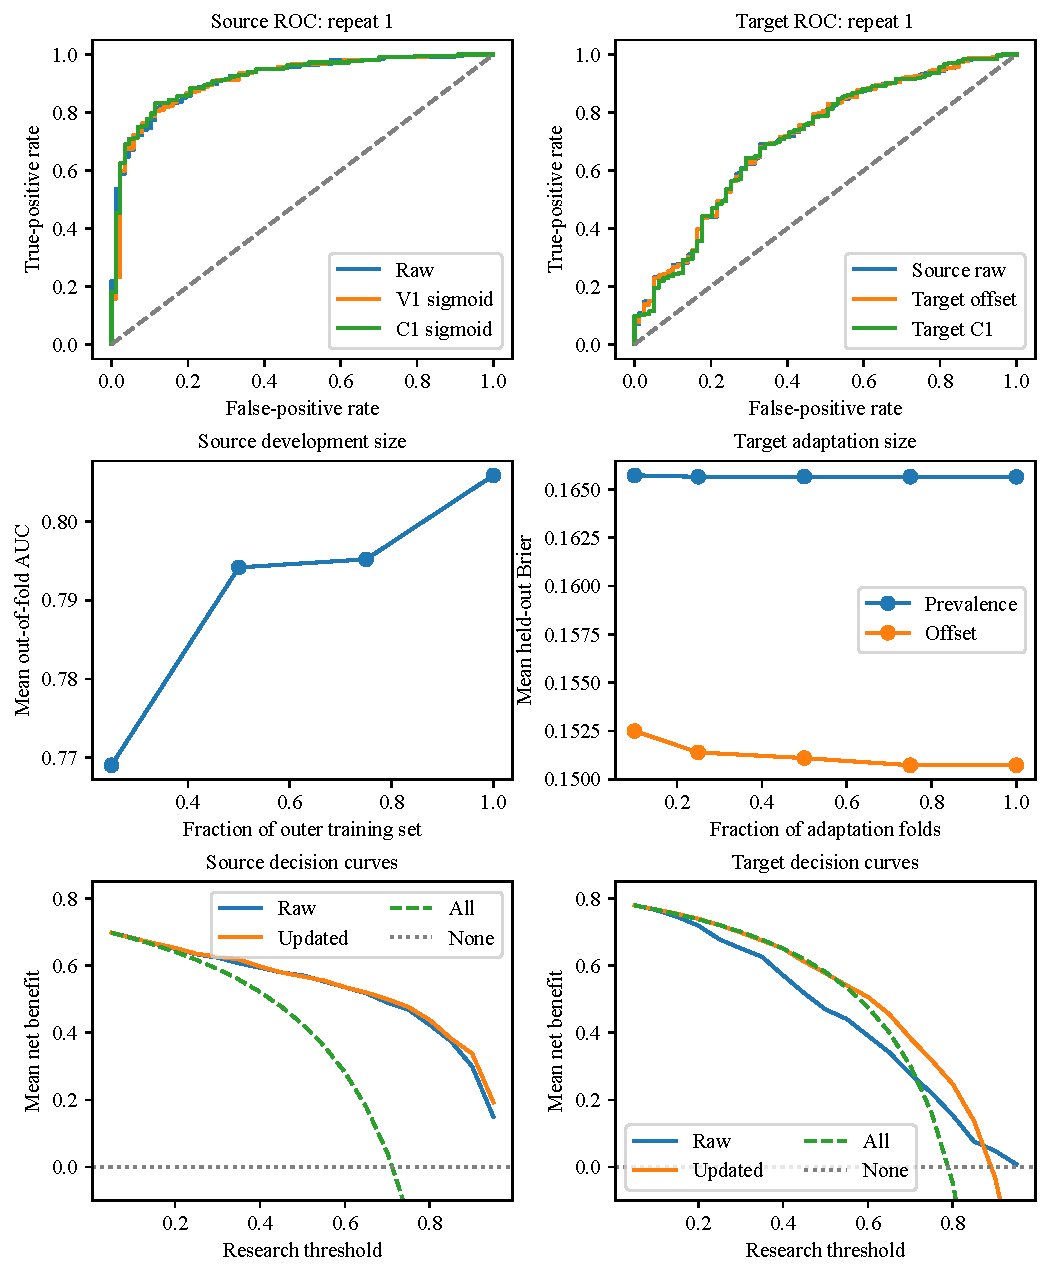
\includegraphics[width=\textwidth]{FINAL_ANALYSES.pdf}
\caption{Final retrospective study overview. Top: repeat-one ROC curves. Middle: development-size and target-adaptation learning curves, averaged across complete repeats. Bottom: exploratory decision curves; the displayed net-benefit axis is limited to $[-0.1,0.85]$ for readability, while all values are retained in CSV. No clinical threshold is recommended.}
\end{figure*}

\begin{thebibliography}{10}
\bibitem{r1} M. J. Khan, B. Raza, and A. Nadeem, "CardioDiag: a machine learning approach for cardiovascular disease diagnosis using XAI-guided hybrid dimensionality reduction and optimized-based ensemble classifiers," PeerJ Computer Science, vol. 12, e4059, 2026, doi: 10.7717/peerj-cs.4059.
\bibitem{r2} G. C. Cawley and N. L. C. Talbot, "On over-fitting in model selection and subsequent selection bias in performance evaluation," Journal of Machine Learning Research, vol. 11, pp. 2079-2107, 2010.
\bibitem{r3} R. Alizadehsani, M. Roshanzamir, and Z. Sani, "Z-Alizadeh Sani," UCI Machine Learning Repository, dataset, doi: 10.24432/C5Q31T.
\bibitem{r4} M. S. Hosseini et al., "AngioCAD: A Publicly Available X-ray Angiography Dataset for Coronary Artery Stenosis and CAD Detection," Zenodo, dataset, 2025, doi: 10.5281/zenodo.15826856.
\bibitem{r5} B. Van Calster et al., "Calibration: the Achilles heel of predictive analytics," BMC Medicine, vol. 17, art. 230, 2019, doi: 10.1186/s12916-019-1466-7.
\bibitem{r6} G. S. Collins et al., "TRIPOD+AI statement: updated guidance for reporting clinical prediction models that use regression or machine learning methods," BMJ, vol. 385, e078378, 2024, doi: 10.1136/bmj-2023-078378.
\bibitem{r7} K. G. M. Moons et al., "PROBAST+AI: an updated quality, risk of bias, and applicability assessment tool for prediction models using regression or artificial intelligence methods," BMJ, vol. 388, e082505, 2025, doi: 10.1136/bmj-2024-082505.
\bibitem{r8} R. D. Riley et al., "Evaluation of clinical prediction models (part 2): how to undertake an external validation study," BMJ, vol. 384, e074820, 2024, doi: 10.1136/bmj-2023-074820.
\bibitem{r9} R. D. Riley et al., "Evaluation of clinical prediction models (part 3): calculating the sample size required for an external validation study," BMJ, vol. 384, e074821, 2024, doi: 10.1136/bmj-2023-074821.
\bibitem{r10} A. J. Vickers and E. B. Elkin, "Decision curve analysis: a novel method for evaluating prediction models," Medical Decision Making, vol. 26, no. 6, pp. 565--574, 2006, doi: 10.1177/0272989X06295361.
\end{thebibliography}
\end{document}
